\chapter{A Field Trip into Sentiment Architectures}
\label{chapterlabel6}

\section*{Chapter summary}

This chapter will present the conducted case studies in support of the research questions. I will introduce two pre-studies of explorative nature, which originally emerged during my MSc studies and before entering a PhD programme. Its promising results laid the ground for the subsequent studies presented here. Based on the outcome we undertook five in depth studies.  All studies are based on the same digital technology to mediate human interaction, but differ significantly in the surface of choice and socio-spatial setting they are embedded within. In describing these case studies, I explore the deployment of each MAI and highlight the implications for designing interactions. The focus is on mediated interactions in the vicinity of the deployed MAI. All case studies differ in the architectural scale and the nature of the urban space (i.e. pedestrianised courtyard vs. congested high street). \newpage



\section{Summary of studies}

The applied research in this dissertation is founded on a series of design projects I have conducted in collaboration with artists, designers and creative technologists (see page \pageref{sec:projects}).
Since 2011 we have invented, developed and implemented seven major projects which I have utilised as studies for this research.

The idea for ordering the studies follows the idea of aligning the different types of surfaces we have been approaching in a chronological order, starting with the smallest surfaces (i.e. DIY display) that has been used in the VEIV study and finishing with a temporary media architecture (i.e. VIVID). 

The focus will be on the \textit{technical}, \textit{social} and \textit{spatial} aspects whilst the weighting of each aspect within the projects is different. Whilst for instance the focus in the ARUP study is on the technical issues we focus on the spatial issues in the RIGA and LINZ study.

\begin{table}[h!]
\centering
\resizebox{\textwidth}{!}{
\setlength{\extrarowheight}{8pt}
\begin{tabular}{l|c|c|c|c|c|c|c}
\hline
\multicolumn{1}{c|}{} & \multicolumn{2}{c|}{Pre-Study}    & \multicolumn{3}{c|}{Study I}                            & \multicolumn{2}{c}{Study II}          \\
\multicolumn{1}{c|}{} & \multicolumn{2}{c|}{Swipe I like} & \multicolumn{3}{c|}{Smart Citizen Sentiment Dashboard}  & \multicolumn{2}{c}{Sentiment Cocoon}  \\ \hline
\multicolumn{1}{c|}{} & SIL                 & VEIV        & RIGA              & SAOP              & LINZ            & ARUP              & VIVID              \\ \hline
date                  & 20.07.-20.08.2011   & 14.06.2013  & 14.11.-18.11.2014 & 12.09.-30.09.2013 & 4.09.-7.09.2014 & 22.05.-28.08.2015 & 27.05.-,18.06.2016 \\ \hline
opening hours         & 1pm-5pm             & 8pm-10pm    & 6pm-11pm          &                   & 9pm-10pm        & 24/7              & 6pm-11pm           \\ \cline{1-7}
achieved hours        & 68h (100\%)         & 3h (100\%)  & 25h (100\%)       & 14h (37\%)        & 16h (100\%)     & 2352 (100\%)      & 80h (70\%)         \\ \hline
total interactions    & 249                 & -           & 2125              & 595               & 910             & 1874              & -                  \\ \hline
single users          & 118                 & -           & 168               & 117               & 75              & 485               & -                 
\end{tabular}
}
\caption[Overview of conducted design studies]{Overview of conducted design studies including the types of electronic surfaces.}
\label{summary_study}
\end{table}




\section{Pre-studies}

The following two studies are labeled as \textit{pre-studies}. The first one (SIL) has been part of my MSc thesis and laid the foundation for this PhD research through the design and implementation of a shared and tangibel user interface in a museum. The second pre-study (VEIV) has been used to explore the potential of turning the MSc research onto PhD level through connecting the interfaces to a self-made architectural surface.

\subsection{SIL - Swipe I like}


\subsubsection {Introduction} 
\subsubsection {Objectives} 
\subsubsection {Methods}
\subsubsection {Implementation}
\subsubsection {Findings and Discussions}
\paragraph{Design recommendations}
%look into Joerg Mueller's paper Looking Glass

This pre-study explores the novel situation and design space that emerge through implementing the popular digital \textit{I Like} button as a ‘tangible and situated interface’ that connects the location of a museum in the real world with online communities. 
The study has been conducted at the UCL Petrie Museum, to the end of investigating the potential of geographically tagging of people’s likes and dislikes, which at that time has been expressed mainly in a digital form through social network applications such as Facebook. 
The aim of this initial study was to explore whether we can enhance the engagement of museums visitors with exhibition content through implementing situated and shared digital technologies in public space. 
Hence we designed and implemented a novel tangible interface (i.e. physical \textit{I like} button) in a museum space that lets people share their views about exhibition content with their digital networks. At the same time we were observing visitors' practices and behaviours when engaging with museum content through the interactive system. 
Our initial findings suggest that implementing tangible devices in museums to enable visitors to voice their opinion about the content enhances engagement and reveals emergent social behaviour. 
The iterative design process and its implementation in a real world context, together with feedback collected and our observations serve to highlight the potential for a location-based social network application based on people’s preferences in the real world.
However the lack of immediate user feedback in form of a display was missing.

\subsubsection{The Technology - The \textit{I like} button}



\subsubsection{The Social -  }

The museum engages actively with issues related to implementing new technologies in the museum setting and showed a particular interest in integrating digital technologies for engaging visitors with their exhibition space.
In consultation with the museum manager we attached the following questions to the devices in order to let people know what to voice their opinion on:

(1) Museum experience
- I like the look and feel of the Petrie Museum and think it holds a distinctive place in the museum sector. - I do not like the look and feel of the Petrie Museum because it is dated and claustrophobic.
(2) Digital technologies
- I like 3D models of objects because they allow me to see objects in more detail and from different angles. - I do not like 3D models because they distract you from the objects and you can never learn as much from a copy as from the original.
(3) Human remains
- I like the display of human remains because they place human presence at the centre of our view of the past and provide valuable historical and scientific information. - I do not like the display of human remains because they may offend the cultural practices or wishes of the individual's descendants.
(4) Repatriation
- I like the idea of repatriation and believe that museums should return ancient artefacts to their countries of origin upon request. - I do not like the idea of repatriation because ancient artefacts belong to the world and thus should be on view around the world.

We deliberately asked questions which we thought might provoke visitors and lead to broad discussions about museum content. The aim was to make sure users would use both buttons. Restricting questions to the overall experience of the museum was considered less likely to yield data worth evaluating because it would be impossible to know whether this is behavior or an expression of true opinion.

\subsubsection{The Space - The Petrie Museum}
The study was carried out at the UCL Petrie Museum of Egyptian Archaeology. The museum has a collection of about 80,000 objects including Egyptian and Sudanese archaeology. The collection consists mostly of small pre-historian art and craft works but also includes human remains and sarcophagi of Pharaohs. All objects are exhibited in continuous glass cases which create long corridors. The museum’s space is narrow, but the atmosphere intimate. 

We distributed four 'I like' devices in the museum's space. One at the receptionist's desk (1), the second on a table in front of an LCD screen which shows 3D laser scanned objects, the third one in front of a glass case that keeps a skeleton in an open clay urn and the fourth one in front of a glass case which includes several death masks and an Egyptian wooden sarcophagus. 

\begin{figure}[!h] 
\centering
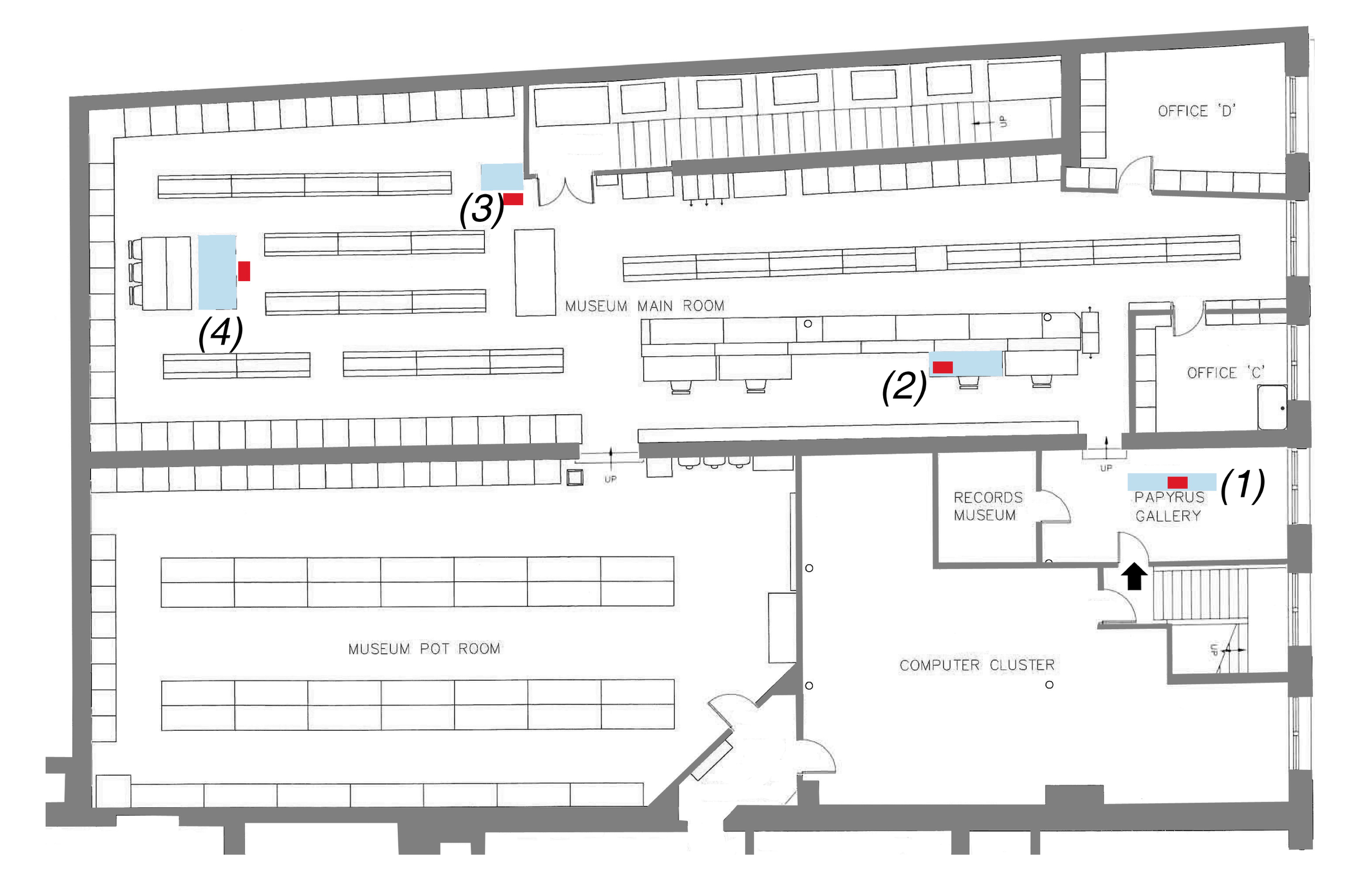
\includegraphics[width=\textwidth]{Illustrations/petrie_layout.png}
\caption [Floor plan UCL Petrie Museum] {Floor plan UCL Petrie Museum including the position of the interfaces: (1) Reception desk + iPad (question about the overall experience in the museum) (2) Desk with LCD screen (question about using digital 3D models on screens in museums) (3) Glass case including human remains (questions about the display of human remains) (4) Glass case showing Egyptian sarcophagus (question about repatriation of ancient artefacts).}
\label{interfaces}
\end{figure}


\subsubsection{Findings}

We started with data collection on Tuesday 20th July 2011 and finished on Saturday 20th August 2011 which means we collected data for five weeks, 25 days in total.

\subsubsection{Discussion}
The findings suggested that visitors are keen to leave their feedback and share it with others (in this case through a simple swipe card interface connecting to Twitter and Facebook).
Analysis of the submitted data discovered movement and encounter patterns of visitors interacting with the installed devices and the observations of interactions revealed various forms of human behaviour such as strangers discussing the purpose of the new interfaces. 
In other words, the space around the tangible device turned into an encounter stage that did not exist at this place before. However, it became clear that a real-time visualisation or representation of the gathered data shown to the audience as an immediate feedback of their actions was desired by many participants but missing in this initial implementation.


\subsection{VEIV - Swipe I like at VEIV London}


\subsubsection {Introduction} 
\subsubsection {Objectives} 
\subsubsection {Methods}
\subsubsection {Implementation}
\subsubsection {Findings and Discussions}


The second pre-study \cite{Behrens_2013} follows-up on the previous implementation we conducted using a TUI of the digital ‘I like’ button, situated in the physical space within a museum context \cite{Behrens_2011} \cite{Behrens_2011b} . 
Building on initial findings regarding movement and encounter patterns and the lack of a immediate feedback, the purpose of the VEIV London study was to: first, explore whether a feedback device that works in a condensed indoor public space can also be deployed in an outdoor public setting full of urban distractions, and second, add a dynamic display to the device to fulfil the need of providing the user with an immediate visual feedback. 
Consequently, we ask what kind of social interactions and dynamic relations of human behaviours take place in an urban setting when mediated by this interactive installation.

\textbf{Technical details and set up}

The LED display consists of three low-resolution displays following the principle of 16 digit number displays, which allow the projection of numbers and letters.
In total, 48 RGB 24V LED light strips (non-addressable) (144 RGB channels) are connected to micro-controllers, which are addressable through the DMX protocol. A decoder transfers the DMX signals through a USB wire to a laptop. The visualisations are programmed with processing. The fact that the lightweight frames are easily movable makes this project easily adaptable to other locations.




\subsubsection{The Space - The Building Projection Party}
The study took place during the UCL Virtual Environments, Imaging and Visualisation doctoral centre (VEIV) festival, 2013, where we set up the first prototype of the LED display at the UCL main campus. 
The installation was running between 8 and 10 pm on a summer day. 
To explore interactivity, we connected the light installation to the binary feedback device based on Radio Frequency IDentification (RFID) technology, which was used in the indoor public space of the museum \cite{Behrens_2011} (Behrens 2011b). During the festival, participants were able to leave their feedback in a playful way through swiping their travel cards (Oyster) or UCL access cards over the thumbs-up or thumbs-down icons on the card reader.
Basically, the simple but effective question was whether visitors like or don’t like the VEIV Centre. When swiping across the thumbs-up icon, the light installation turned the VEIV logo into a warm orange, whilst the thumbs-down icon turned the logo into a cool blue.

\begin{figure}[!h] 
\centering
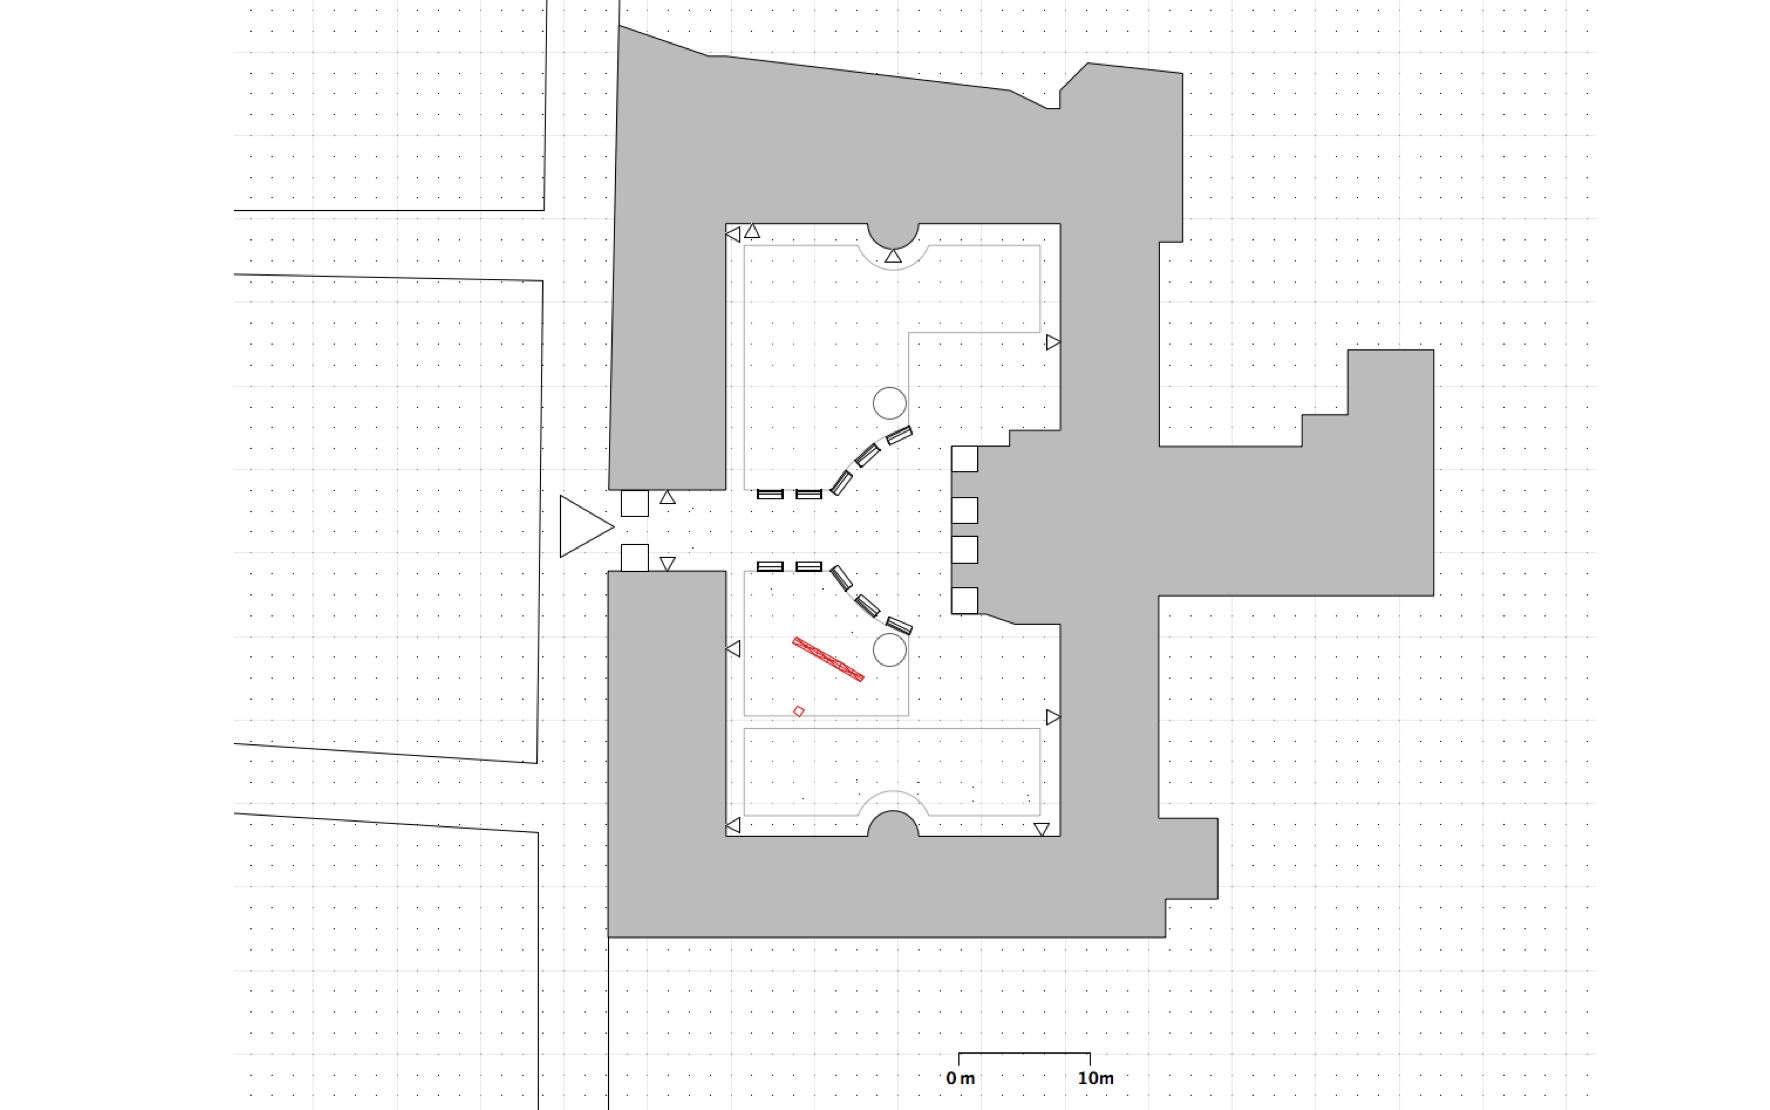
\includegraphics[width=\textwidth]{Illustrations/VEIV_floorplan.png}
\caption [Floor plan UCL Main Quad] {Floor plan UCL Main Quad during the VEIV party including the position of the DIY display and the interface (both in red).}
\label{VEIVfloorplan}
\end{figure}


\begin{figure}[!h] 
\centering
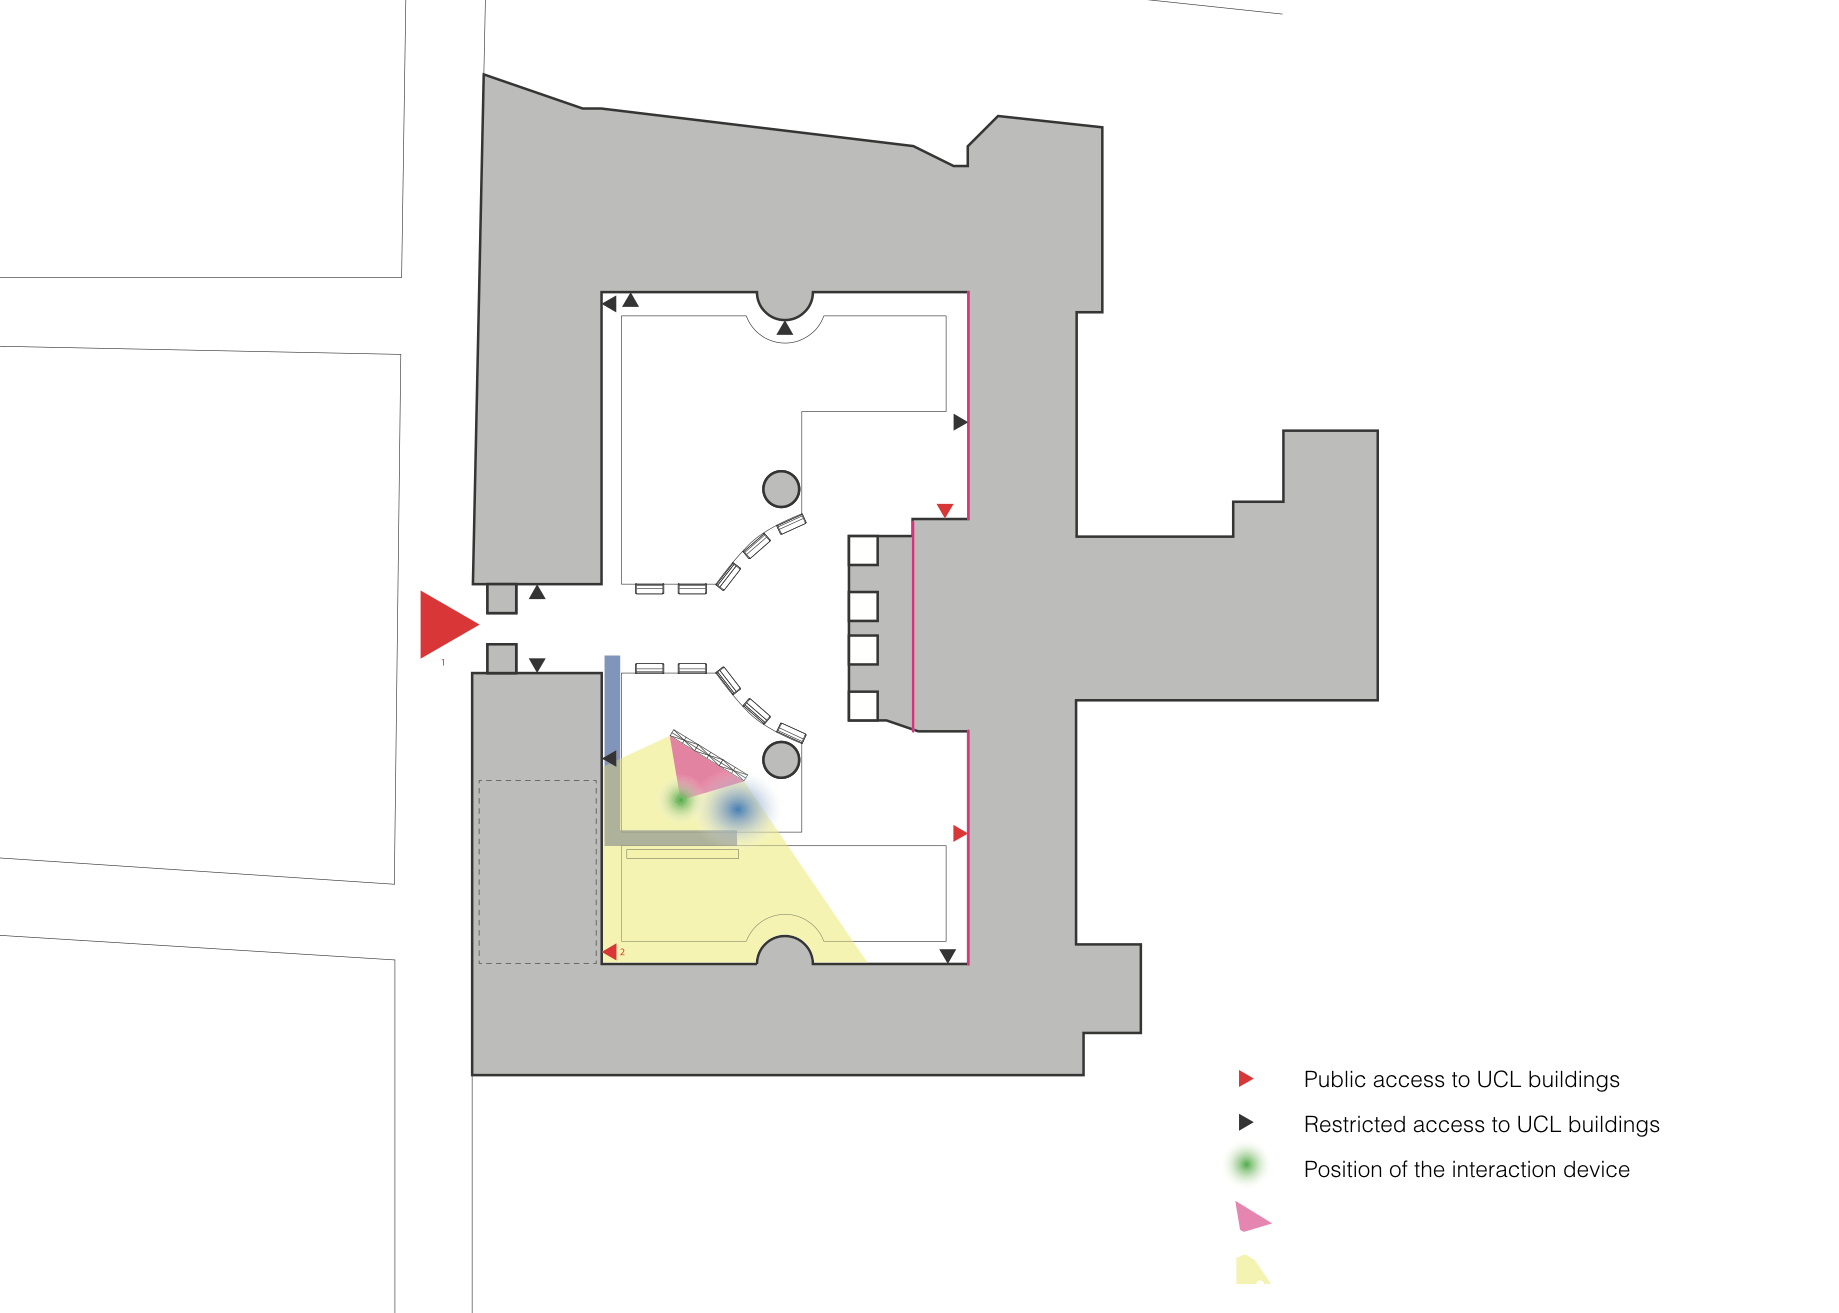
\includegraphics[width=\textwidth]{Illustrations/VIVEinteractionspaces.png}
\caption [VEIV interaction spaces] {VEIV interaction spaces.}
\label{VEIVinteractionspaces}
\end{figure}




\textbf{Observations}

During the first hour, the daylight reduced the light distribution of the LED light, whereas with the approaching darkness the LEDs were colouring the surrounding buildings in either orange or blue ambient light.
Throughout the event, we took pictures, notes and informally talked to people joining the event. Overall, participants liked the idea and enjoyed using their Oyster Cards or UCL access cards to change the colour of the low-resolution display. However, the fact that they were actually rating the event was less important than the playfulness of changing the colours.
We observed people sitting on the lawn suddenly walking up to change the colour from the apparently uncomfortable blue to the warm orange. They obviously felt more comfortable with the cosy orange light than with the cold blue light.
A kind of camp-fire atmosphere was created where people were sitting around a source of pleasant light that illuminates the faces of others as well as putting the surrounding facades of the classic campus building into an orange-red shade.
The lawn in front of the installation was the preferred seating area and the TUI (i.e. ‘I like’ device) created a stage for social encounters. However, after sunset, people moved away from the immediate space around the display as the LEDs became too bright. 

\begin{figure}[!h] 
\centering
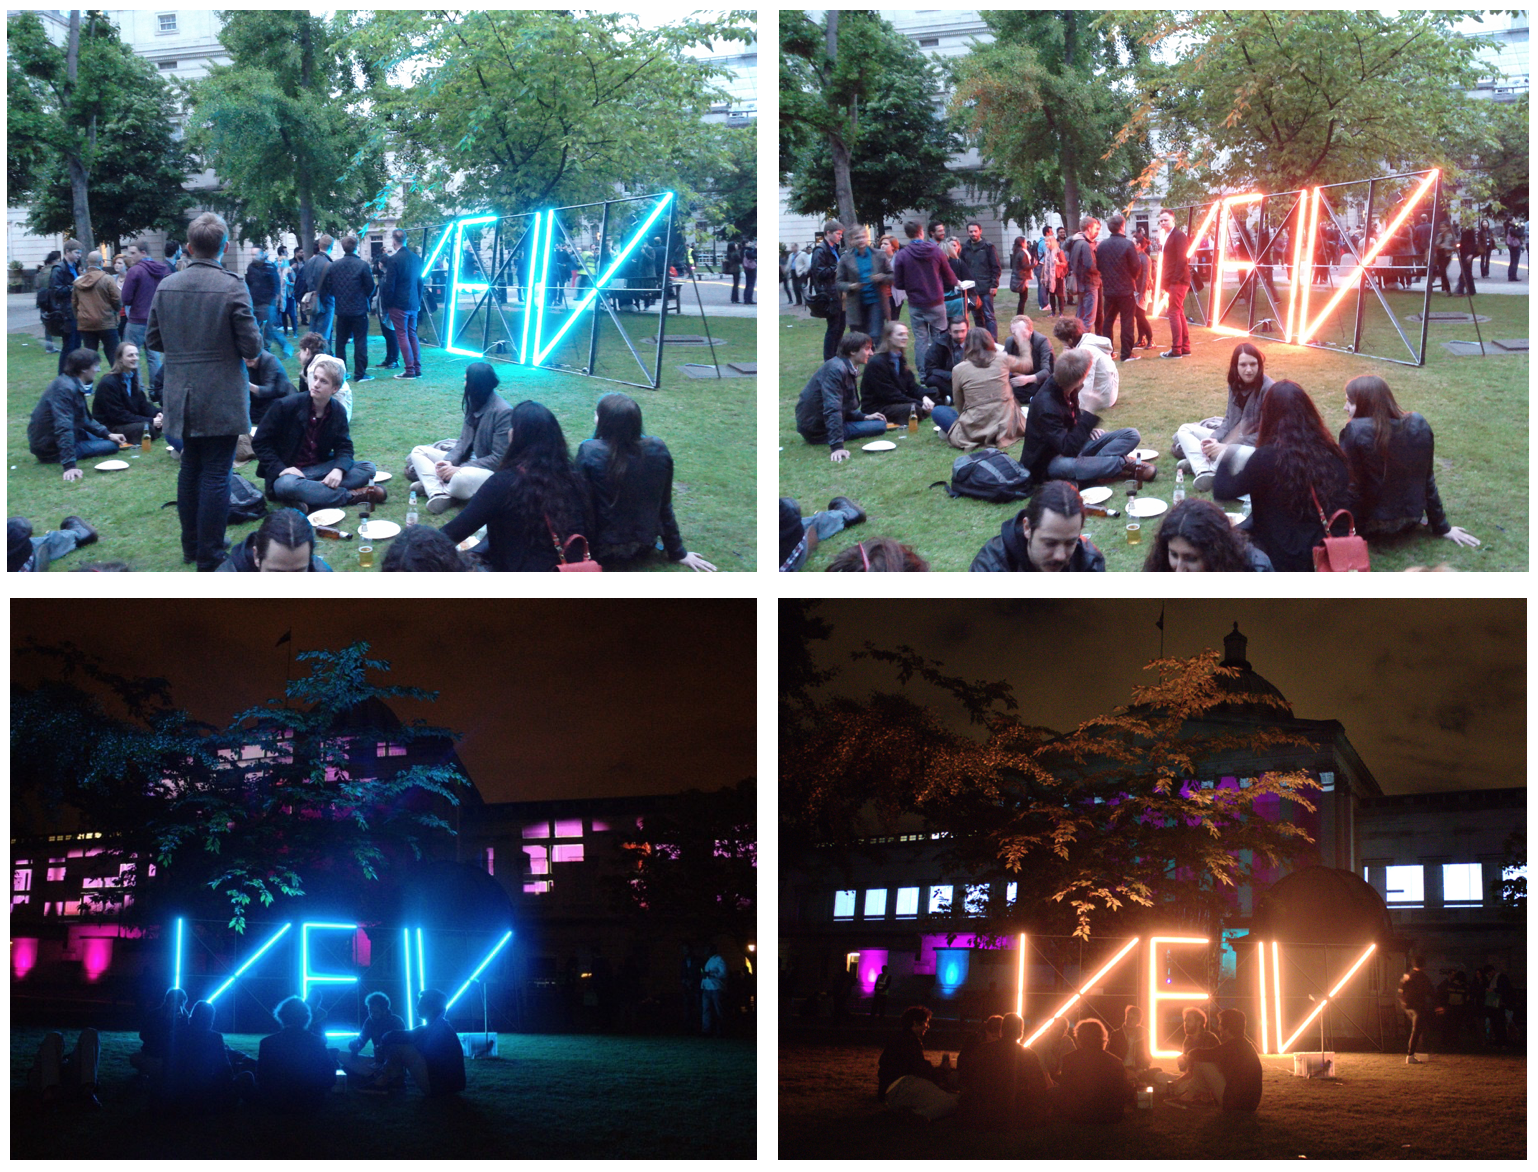
\includegraphics[width=\textwidth]{Illustrations/VEIVcampfire.png}
\caption [Campfire atmosphere] {camp-fire atmosphere was created where people were sitting around a source of pleasant light that illuminates the faces of others.}
\label{VEIVcampfire}
\end{figure}

Interestingly, people neither sat nor stood in between the tangible interface and the LED display nor behind the LED display.
The DIY and low-resolution media display worked out very well considering the relatively low effort that was put into the design and making of the low-resolution screen and the visual impact of illuminating a courtyard during a large public
event was huge. 

\textbf{Summary of pre-studies}

With the two pre-studies described I explored the potential for novel digital technology to be placed in the public realm as a mediator for social interactions. I identified challenges regarding system architecture (i.e. technology needs to provide immediate feedback for users) and spatial settings (i.e. the difference between closed indoor space of a museum versus the condensed outdoor space of a university campus).
Based on these initial findings the case studies have been scaled up in their technological set up and the duration of their implementation.  

\section{SCSD - Smart Citizen Sentiment Dashboard }

The Smart Citizen Sentiment Dashboard (SCSD) is an interactive participatory installation that lets citizens engage with, and comment on, urban challenges in their cities. 
Through a tangible interface connected to a large electronic surface such as \textit{Urban Screens}, \textit{Media Facades} or \textit{Media Architecture}, passersby and participants on-site can submit their sentiments and simultaneously see the effect of their actions projected onto the \textit{Surface}. 
The tangible urban interaction device allows for an intuitive and accessible, yet identifiable and public way of expressing ones view. 
The project aims to create an open, aesthetic dialogue about urban challenges and invites citizen to engage, by playfully allowing them to express their opinion and share and compare their views in the physical built environment.

The Smart Citizen Sentiment Dashboard project comprises three studies. 
These studies have a common design concept, which has been implemented in three different temporary media art festivals. 
The concept idea follows the two pre-studies in the way that we have implemented a feedback device that allows people to express their sentiments. 
These devices have been further advanced during each occasion. 
The kind of display for immediate feedback projection changed each time, beginning with a mobile \textit{Urban Screen} in Riga, followed bt a large \textit{Media Facade} in Sao Paulo and a \textit{Media Architecture} in Linz.  

\subsection{RIGA}

\subsubsection {Introduction} 
\subsubsection {Objectives} 
\subsubsection {Methods}
\subsubsection {Implementation}
\subsubsection {Findings and Discussions}

During the Staro Riga Festival in Riga, Latvia the installation was set up on a busy pedestrian crossing at the intersection of Marijas Iela and Satekles Iela, which is close to the Riga main train station. The visualization was displayed on a large mobile screen facing towards Satekles Iela, and the sentiment dashboard was set up in front of it. The installation ran daily in between 6pm and 11pm starting Friday, 14 November 2014 and finished at the National Independence Day on Tuesday, 18 November. During the five days of deployment, in which the installation was running for five hours each evening, the interactive system tracked approximately 1600 interactions.

\begin{figure}[!h] 
\centering
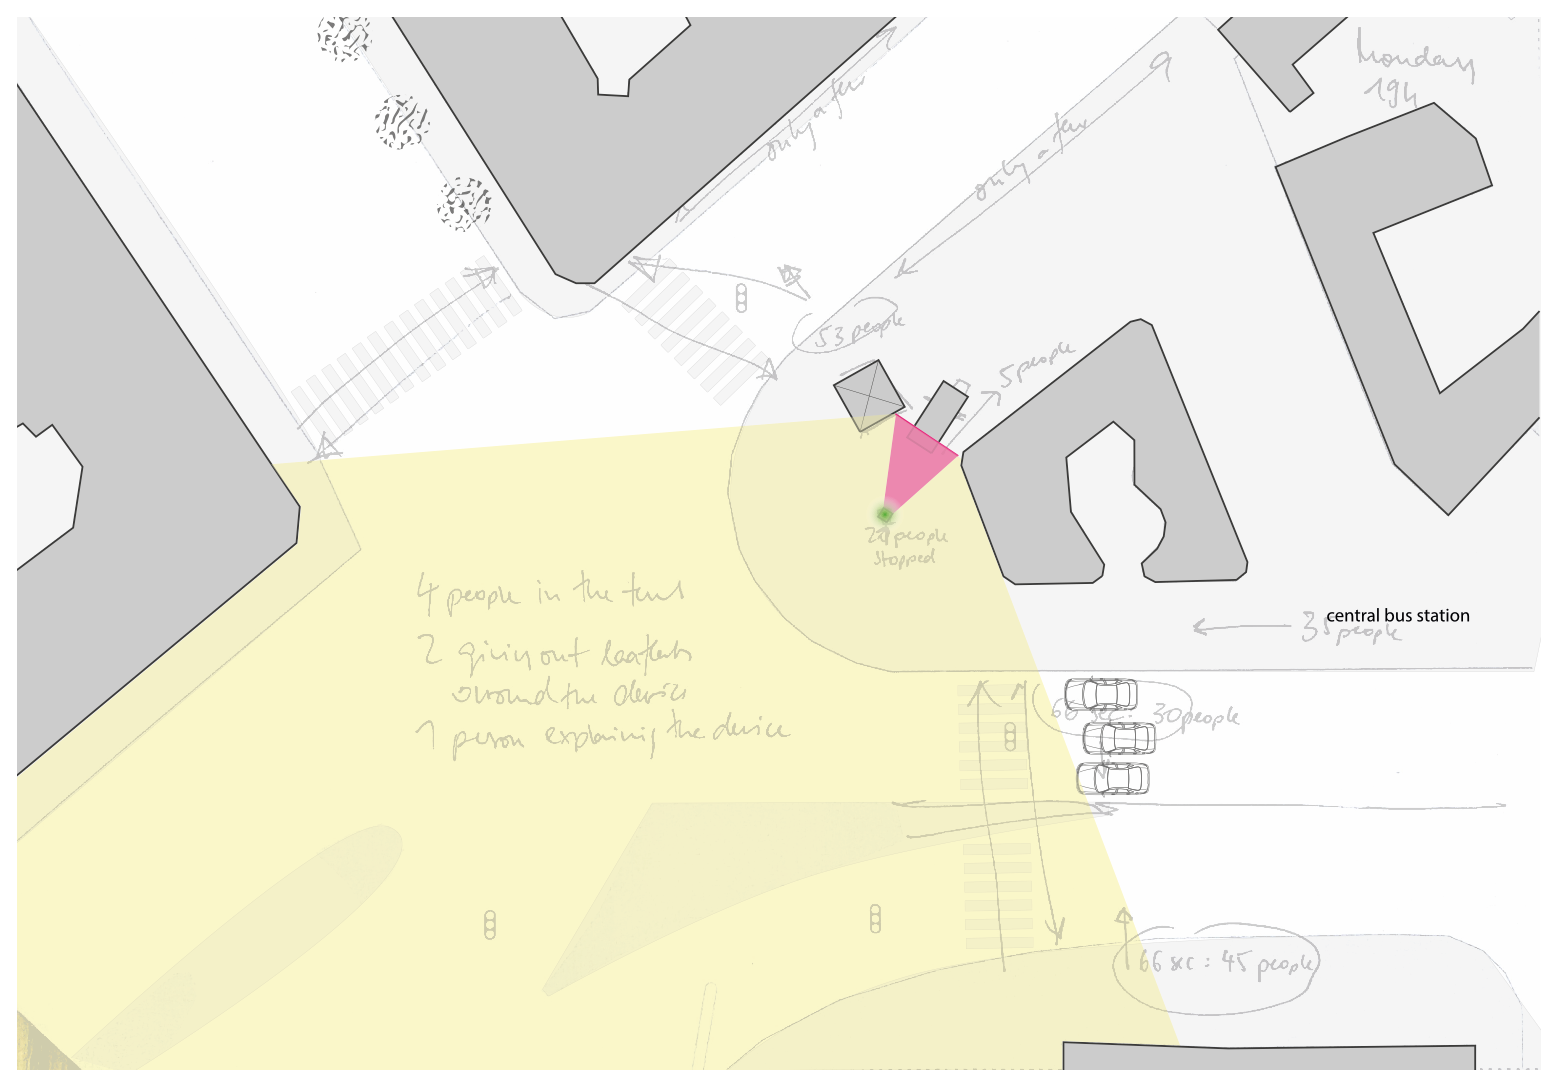
\includegraphics[width=\textwidth]{Illustrations/RIGA_floorplan.png}
\caption [Floor plan RIGA] {Floor plan RIGA.}
\label{RIGAfloorplan}
\end{figure}

\subsubsection{The Dashboard}

The motivation was to develop, design and deploy a situated and tangible system that mediates collaborative interactions in public spaces. 
The employed technology makes use of existing ‘Radio frequency identification’ (RFID) as known from smart card technology such as the e-talon in Riga. 
We build on the widely spread use of these unique ID tags for payless travel purposes, as a large proportion of citizens of Riga carries an e-talon in their pocket. 
Consequently the use of these cards is a recurring embodied interaction in the smart city. 
At the same time every interaction is uniquely identifiable and therefore traceable. 
Our aim was to allow people to use their ID tags beyond technical purposes and express their mood and opinion about specific issues in the technology mediated urban realm. 
Hence the Smart Citizen Sentiment Dashboard (SCSD) enables participants to express their mood about urgent urban challenges in the city of Riga. 
The challenges were defined as follows: 1) ATTĪSTĪBA (development), 2) TRANSPORTS (transport), 3) VIDE (environment), 4) DROŠĪBA (safety) and 5) KULTŪRA (culture). 
By switching a knob on the device participants are able to choose one of the aforementioned categories. By swiping their RFID token (i.e. e-talon) across one of the two emoticons (happy or sad) their mood was transmitted onto the LED display. 
The SCSD affords three folded interactions: 1) switching: 5 categories can be selected through a rotary switch; 2) swiping: after choosing the category, the electronic ID card needs to be swiped over one of the three mood states (happy, indifferent, sad); 3) pushing: finally a simple push-button (Red Button) allows users to view the overall feedback of all collected moods.

\subsubsection{The Visualisation}

We chose a visualisation technique that combines the “seriousness” of the topic with the more accessible style of popular info-graphics. 
The visualisation consists of an abstract sunburst representation, of which each burst corresponds to the sentiment of an individual participant towards the currently selected urban challenge. 
Each urban challenge is encoded by a different colour and an icon representation. 
Upon switching the rotary knob, the sunburst visualisation corresponding to the specific urban challenge, and coloured accordingly appears on the facade.

The sentiment ‘value’ for each participant (happy, un-happy) is graphically encoded through the length of the corresponding burst: the longest burst represents a positive sentiment towards the urban challenge at hand, while the shortest corresponds to a negative statement. 
Our choice for this circular visualisation technique was also motivated by its scalability, which allows for an arbitrary number of people to participate and be visually represented. 
We considered this flexibility a desirable feature in the context of urban environments, often characterised by highly variable and open-ended, and unpredictable flux of people and interactions.

\subsubsection*{Animations}

The integration of dynamic visual cues can make visualisations richer, more vivid and therefore easier to understand. 
Accordingly, our visualisation shows a dynamically animated circle over the sunbursts in order to convey the average participants’ sentiment for the given urban challenge. 
Each new burst from a participant visually appears with a smooth animation and bouncing effect, to highlight the recording of fresh data. 
A new entry is displayed in a white color to unambiguously distinct it from the rest of the graphical representation. 
Shortly after it is smoothly taken over by the color of its respective urban challenge.

\subsubsection*{The Red Button}

In order to provide citizens with an overview of previously submitted sentiments, and a more interactive approach to exploring the installation, we integrated a ‘Red Button’ at the bottom of the interface. 
When pushing this button, a dynamic visualisation of the average feedback for all available urban challenges is represented on the facade. 
As mentioned above, each urban challenge is represented by its corresponding colour, and occupies a different part of the circular shape proportionally to the relative participation rate of the according challenge. 
We aimed to create a simple, playful, yet meaningful approach to enable citizens and participants alike to make a deeper sense of the installation, and the underlying participation results: people can gain insight about which urban challenge is most attractive to vote for, and what is the average sentiment about it of fellow citizens. 
This, beyond being an overview, the heart visualisation symbolises the overall ‘sentiment’ of the city towards its urban challenges.

\subsubsection{Riga’s Sentiments}

The installation was running for five days, in total for 25 hours. During this time the database logged about 1600 interactions.
These interactions cannot automatically be counted as single votes by individuals as many participants were exploring the installation in a playful manner through swiping their e-talon more often.
In a next step with an elaborate data cleaning process this behaviour can be removed from the data set. 
However, we can already identify a clear tendency that shows that participants overall voted positive, as 75 percent of the interactions were happy. 
If we look more closely into the different urban challenges we can reveal more telling insights of how the citizens of Riga think about their city. 
ATTĪSTĪBA (development) was the category, which attracted with 356 interactions the least attention of participants. 
Still 76 percent (270 counts) of the recorded data was positive. 
As development maybe interpreted in many ways participants could have felt irritated and therefore may have decided not to vote in this category. 
TRANSPORTS (transport) and DROŠĪBA (safety) were the most controversial topics, which is by the way in line with other cities where the installation was running before. 
Transport attracted 379 interactions and safety 434 interactions of which both topics were 65 percent happy and 35 percent un-happy. 
As there were more interactions tracked for the category of safety one may argue that this is due to the higher importance of this topic to participants. 
VIDE (environment) attracted 447 interactions of which 78 percent were positive and 22 percent negative. 
KULTŪRA (culture) has been the topic most participants wanted to express their sentiments about. 
The system logged 518 interactions of which 441 (85 percent) were positive and only 77 (15 percent) negative. 
Culture is therefore not only the most frequently used urban topic but also the topic participants are the happiest about. 
One may argue that this result might be due to the fact that participants were influenced by the many cultural events that were going on at this time during the Staro Riga Festival.

\subsubsection{Observations}

Overall it is to say that the logged interactions by the system were on average 75 percent positive as well as none of the categories reached a majority of un-happy interactions. This is a result we did not find in any previous deployment and therefore lets us assume that Riga is a city where people seem to be quite content with the addressed urban challenges or tend to see things in a rather positive way.

Our observations revealed three different participation patterns:

\textbf{The serious behaviour}

A participant submits exactly one sentiment for each of the explored categories. 
This pattern would reflect how we expected the interaction mechanism to work – i.e. a person would explore the categories by rotating the knob and would submit one sentiment for a specific preference.

\textbf{The repetitive behaviour}

This was the most frequently observed participation pattern. The participant has submitted the same sentiment (same preference for a certain category) several times within the considered time range. The occurrence of this pattern can be explained with our frequent observation of participants holding their card over the RFID reader (for a certain preference) for several seconds. Thus the system registers several submissions (although our system had restricted votes not to be registered within 5 seconds after each given participation). This behaviour might be due to a usability flaw of our installation – the participating person did not realize the effect of her participation in the visualization, hence tried several times. Another explanation might be the manifestation of a particular sentiment towards one urban challenge: by holding the card over the reader, the user might have wanted to reassure herself that her opinion would be registered by the system.

\textbf{The playful behaviour}

There were many occurrences of this behaviour during the deployment of the installation. The participant has submitted several different preferences for the same category within the considered period of time. This might indicate that s/he did not really want to express an opinion, but rather explored how the installation and the visualization work. While we cannot account for representative polling results, the findings indicate the installation fulfilled its intentions as an urban feedback platform, where people engage meaningfully with locally relevant topics. In the future it would be exciting to deploy several citizen sentiment dashboards permanently across the city as well as working closer with city authorities and local communities. This might open a fruitful dialog in between citizens and stakeholders of Riga.

\subsubsection{Discussion}



\subsection{SAOP - Sao Paulo}

\subsubsection {Introduction} 
\subsubsection {Objectives} 
\subsubsection {Methods}
\subsubsection {Implementation}
\subsubsection {Findings and Discussions}

\subsubsection{Viva Cidade Festival}

Similar to the RIGA study, the employed technology makes use of existing RFID technology by using the Bilhette Unico, the public transport card in Sao Paulo. 
Hence, the Smart Citizen Sentiment Dashboard (SCSD) enables participants to express their mood about urgent urban challenges in the city of Sao Paulo (Behrens et al. 2014).

\begin{figure}[!h] 
\centering
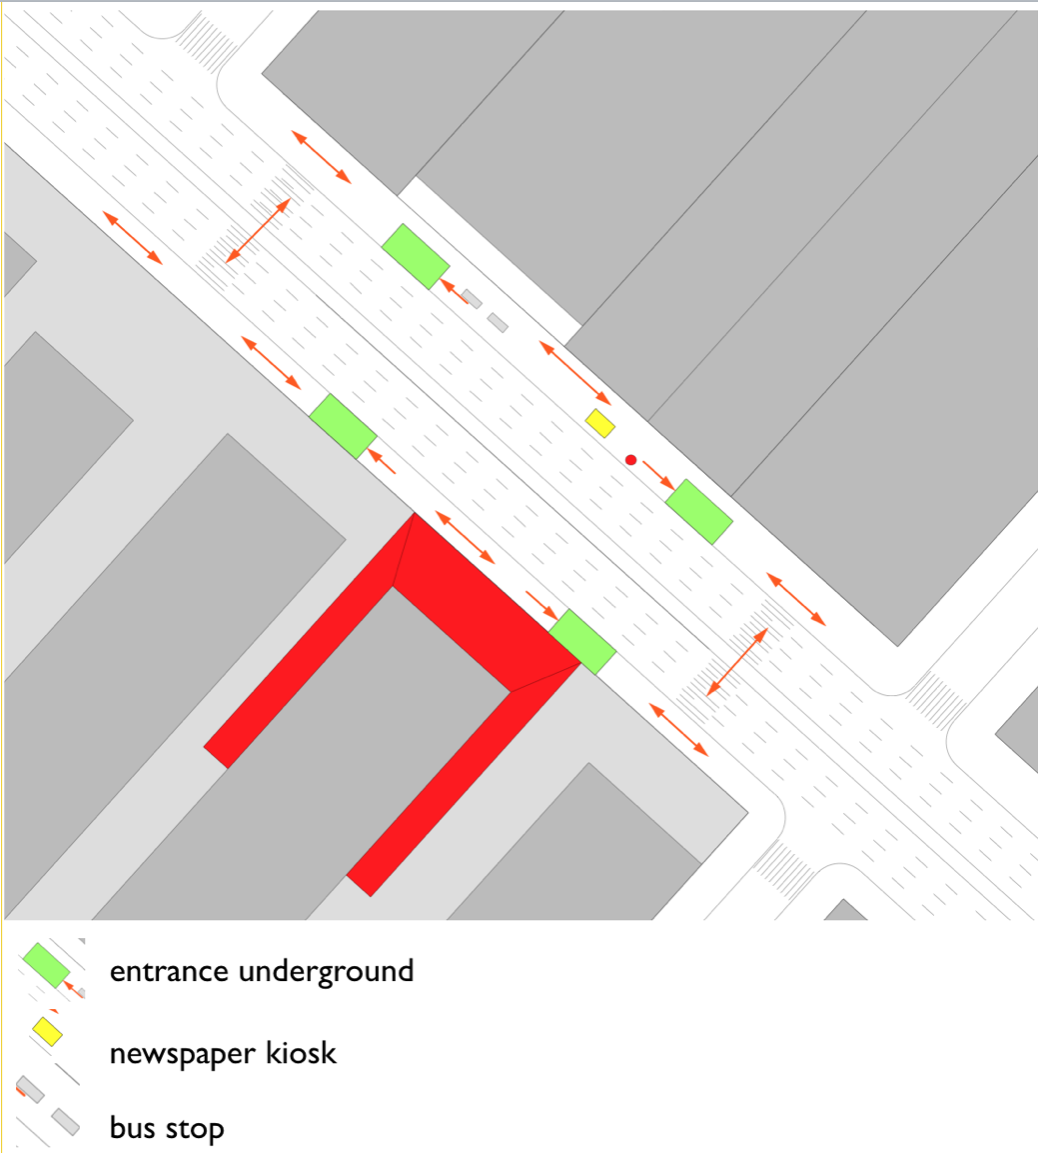
\includegraphics[width=\textwidth]{Illustrations/SAOPfloorplan.png}
\caption [SAOP floor plan] {SAOP floor plan.}
\label{SAOPfloorplan}
\end{figure}

Up front, we were running four design ethnographic workshops amongst various social groups in Sao Paulo with the aim to learn about citizens’ urban challenges. 
As a result of the collaboration, five categories were established: (1) environment, (2) mobility, (3) security, (4) public space and (5) housing.
By switching a knob on the device, participants are able to choose one of the aforementioned categories. By swiping their RFID token (i.e. Bilhette Unico) across one of the three emotions (happy, indifferent and sad), their mood was transmitted on to the media facade (i.e. display).
The mood expressed by the user (i.e. happy, indifferent or sad) is then projected onto a huge LED media facade (i.e. display), which has been retrofitted in the existing honeycomb facade of the pyramidal FIESP building.


The media facade is divided into three parts, which are situated on three different sides of the facade. The biggest and main display faces to the opposite side of the street, whereas the two smaller screens are directed to display to both directions of Avenida Paulista. 
The threefold low-resolution LED facade is formed of a network of approximately 26,000 LED clusters (pixels) embedded in 3700-m2 metal structure that covers the pyramidal FIESP building. 
The grid is approximately 13 × 13 cm. Each pixel consists of a module of four LEDs: 2 × R, 1 × G, 1 × B the luminous intensity is 4.5 cd/module.
 
The visualisation comprises of an abstract sunburst representation, of which each burst corresponds to the sentiment of an individual participant towards the currently selected urban challenge. 
Each urban challenge is encoded by a different colour and an icon representation. 
Upon switching the rotary knob, the sunburst visualisation corresponding to the specific urban challenge and coloured accordingly appears on the facade. 
The sentiment ‘value’ for each participant (happy, indifferent, sad) is graphically encoded through the length of the corresponding burst: the longest burst represents a positive sentiment towards the urban challenge at hand, whilst the shortest corresponds to a negative statement. 
Our choice for this circular visualisation technique was also motivated by its scalability, which allows for an arbitrary number of people to participate and be visually represented.
We considered this flexibility a desirable feature in the context of urban environments, often characterised by highly variable and open-ended, and unpredictable flux of people and interactions. 
The integration of dynamic visual cues can make visualisations richer, more vivid and therefore easier to understand. 
Accordingly, our visualisation shows a dynamically animated circle over the sunbursts in order to convey the average participants’ sentiment for the given urban challenge. 
Each new burst from a participant visually appears with a smooth animation and bouncing effect, to highlight the recording of fresh data. 
A new entry is displayed in a white colour to unambiguously distinct it from the rest of the graphical representation.
Shortly after, it is smoothly taken over by the colour of its respective urban challenge. 
In order to provide citizens with an overview of previously submitted sentiments, and with a more interactive approach to exploring the installation, we integrated a ‘heart’ button at the bottom of the interface. 
When pushing this button, a dynamic visualisation of the average feedback for all available urban challenges is represented on the facade. 
As mentioned above, each urban challenge is represented by its corresponding colour and occupies a different part of the circular shape proportionally to the relative participation rate of the according challenge.
We aimed to create a simple, playful, yet meaningful approach to enable citizens and participants alike to make a deeper sense of the installation, and the underlying participation results: people can gain insight about which urban challenge is most attractive to vote for, and what is the average sentiment about it of fellow citizens. 
This, beyond being an overview, the heart visualisation symbolises the overall ‘sentiment’ of the city towards its urban challenges.

\subsubsection{Findings and discussion}

Our findings suggest that the implementation of a tangible interface not only supports engagement indoor, such as in a museum context, but also outdoor during a festive event and a media art festival. 
Yet, the actual TUI in an outdoor setting was not immediately attracting participants. 
Instead, our observations suggest that the strong visual presence of the display (i.e. low-resolution display or media facade) appealed peoples’ attention first.
In the pre-study, VEIV London, the interactive system consisted of a simple binary RFID swipe card interface. In the study conducted in Sao Paulo, the shared user interface was again based on RFID technology but with additional features such as a rotary knob and a push button. 
Initially, we decided to use RFID technology instead of simple touch buttons due to the potential to identify the user.
We were able to track individual user behaviour such as returning users or misapplication, which simple buttons would not allow. 
Despite these useful features, we observed that the need for an individual swipe card generated a barrier that was hindering some people to interact. 
The reasons for this may be manifold: in London, the use of the transport card (i.e. Oyster Card) has a wider distribution amongst all citizens. 
Public transport is generally considered to be a convenient way of commuting and people feel secure using London buses or undergrounds.
Consequently, the usage of the Oyster Card appears to be more embodied than in Sao Paulo, where private transportation is very common, mostly due to personal security. 
Thus, Londoners more likely understand how to engage with the interface and particularly liked the idea to use a smart card to give feedback about services. 
However, we observed that the fact that not all people carrying a RFID card in their pockets triggered unexpected social encounters during both studies.
Bystanders, curious to get involved, asked actors to borrow their cards, or families sharing one card amongst each other. In addition, bystanders started debating about the sense of having such interfaces in urban space or simply wanted to know how the technology works.
During the SCSD Sao Paulo study, we looked closely at actors directly interacting with the TUI. 
The most common behaviour actors performed started with looking at the TUI, swiping their card or turning the rotary knob. 
After expressing their feelings towards one of the categories at the swipe card interface, we saw that participants would then frequently look up to the media facade to see what impact their acting had on the visualisation. 
The fact that the visualisation was slightly delayed (i.e. less than a second) was an advantage for the actor experience as it left time for the body orientation towards the large media facade. 
Close bystanders were behaving almost synchronic in order to understand the interaction modality.
At the same time, we made observations in the wider surrounding of the MAI during the SCSD Sao Paulo deployment.
We recognised MAI-related interactions around the facade in the close interaction space as well as in the wider ambient space. 
Although these observations were not rigorously conducted, we did notice a few recurring behaviours. In particular, we frequently saw people taking pictures of the media facade with their mobile phones or taking pictures of each other in front of the facade. 
These informal observations would suggest that people simply liked the visual presence of the media facade’s visualisation and the heart icon it used. 
Yet, the initial design aim was to develop an interactive system, which would spark passers’-by engagement with the informational content and eventually may trigger new social encounters and discussions about the matter. 
In the case of VEIV London, participants were asked to express their opinion about the UCL doctoral centre (i.e. like or don’t like), whilst during the SCSD Sao Paulo event contestants could share their sentiments about urgent urban challenges in their city (i.e. environment, mobility, security, public space or housing). 
Accordingly, this raises the question regarding the informational character of the installation as intended and the actual ambient perception of the visualisation by many people in particular outside the direct interaction space in the close vicinity of the TUI.
Our findings here suggest that designers need to take the ambient perception of MAI set ups into account when designing interactive systems in urban environments.

\subsubsection{Conclusion}


\subsection{LINZ - Ars Electronica}


\subsubsection {Introduction} 
\subsubsection {Objectives} 
\subsubsection {Methods}
\subsubsection {Implementation}
\subsubsection {Findings and Discussions}


\subsubsection{Ars Electronica Festival}

The Ars Electronica Center (AEC) display is built into the facade and consists of 1085 illuminated windows each sized ca. 3×1 meters and corresponds to a pixel.
\begin{figure}[!h] 
\centering
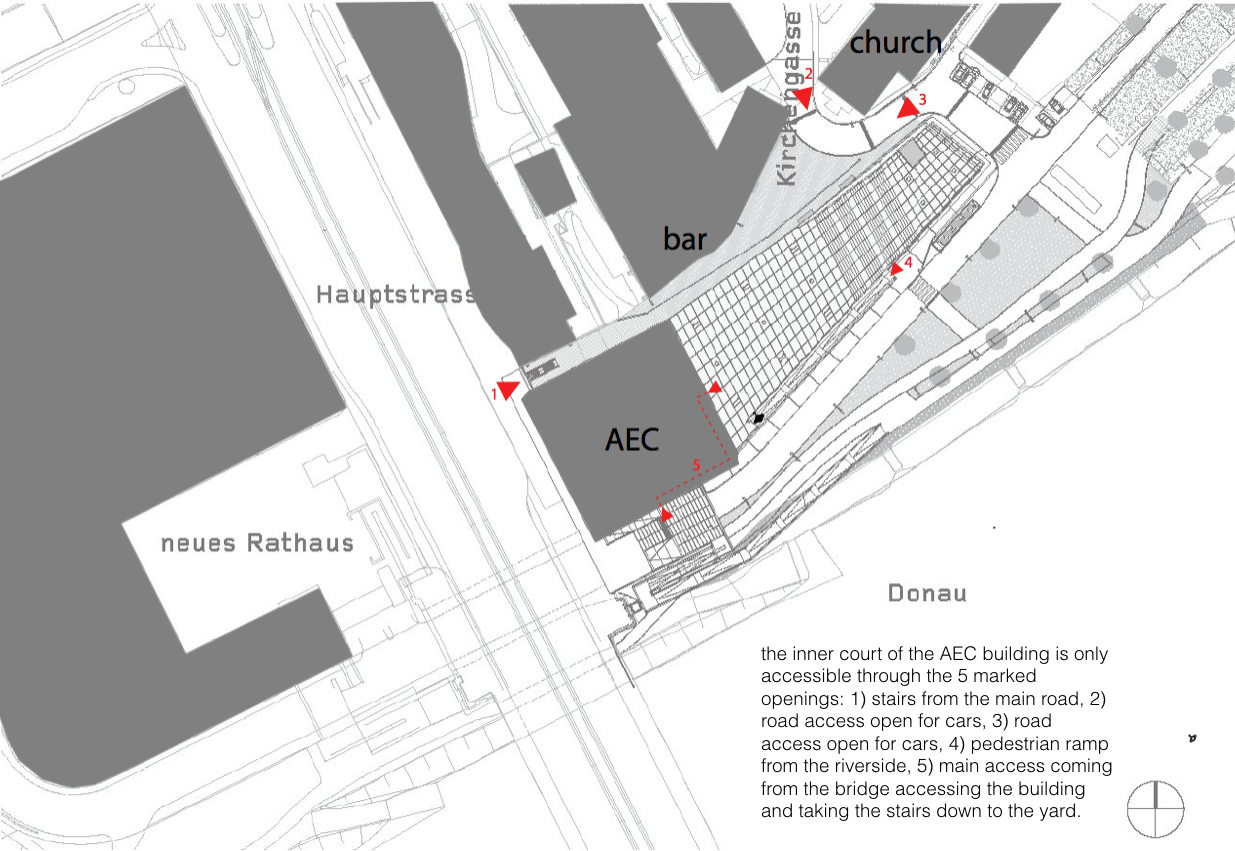
\includegraphics[width=\textwidth]{Illustrations/AEC_floorplan.png}
\caption [Floor plan LINZ] {Floor plan LINZ.}
\label{LINZfloorplan}
\end{figure}
The Sentiment Dashboard was connected to the media façade of the AEC in Linz. 
For the AEC media façade, the SCSD visualization attempted to balance between the ambient character of the low-res façade and the informational goals of the SCSD project. Eventually we designed a ‘star field’-like visual behavior where each pixel (i.e. window in the building) represents a citizen’s sentiment, submitted through the situated dashboard. As each urban challenge is represented through a colour, submitting a positive sentiment towards a given challenge results in the “birth” and “star field” of the visualisation with a “pixel” from the same colour. A negative sentiment is displayed as white light, so that the proportion between positive and negative sentiments for a given topic is clearly discernible. The more recent the submission of a sentiment, the higher the movement speed of the sentiment “representative”. Subsequently, older submissions result in slower movement, and eventually fade out. In this way, we aimed to convey a visual impression on the audience’s behaviour and dynamics towards the installation and its topics, beyond the mere representation of overall results.

\section{Sentiment Cocoon}

\subsection{ARUP - Sentiment Cocoon at Arup, London}


\subsubsection {Introduction} 
\subsubsection {Objectives} 
\subsubsection {Methods}
\subsubsection {Implementation}
\subsubsection {Findings and Discussions}


\subsubsection{No.8@Arup Competition}

The competition, under which the Sentiment Cocoon evolved, called No.8@arup , is a programme that provides space to host installations and sculptures in Arup’s Central London office. 

\begin{figure}[!h] 
\centering
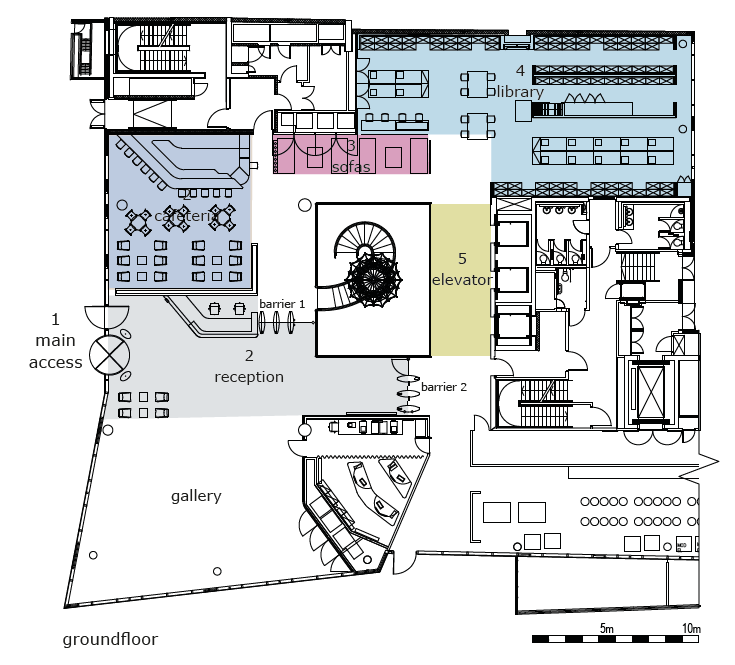
\includegraphics[width=\textwidth]{Illustrations/ARUPfloorplan.png}
\caption [Floor plan ARUP] {Floor plan ARUP: On groundfloor level the following communal facilities are connected to the atrium.}
\label{ARUPfloorplan}
\end{figure}

\subsubsection{Initial design idea}

We propose an interactive cocoon weaved out of a translucent fabric that turns the atrium into a stage for social encounter. The aim is to foster the notion of an atrium as the social centre of a building. Our focus is on the exploration of architectural form, translucent materials and responsive lighting to facilitate social interaction. We collect people’s sentiments and materialise them into light and fibre.
Based on our experience in human-computer interaction and interactive lighting we suggest a system that lets occupants interface with the light structure by using any RFID card. Simple sentiment interfaces attached to the entrance barriers and rails on each floor allow employees to express their current sentiments. These interactive dashboards were designed with knobs, dials and buttons. Each day, Arup people will be encouraged to share their sentiments via one of the dashboards that are installed on each of the six office floors. As people approach the dashboard they will be invited to choose which mood they are in to record their sentiment of the day. People will operate a dial and this will identify their sentiment, happy, sad or indifferent. Individual swipe cards such as the London Oyster card will enable participants to submit their sentiment for the day. As everyone’s RFID enabled swipe card is unique this will allow the system to identify behaviour albeit anonymously. A sophisticated algorithm will feed participants’ feelings through the dashboard and these will be digitally projected into a light field created by LEDs that forms the spine of the cocoon.
Our system architecture allows for the tracking and displaying of several behaviours. These parameters are encoded into lighting patterns that suggest the collective mood of the building’s occupants. The sentiment engine (database) collects human data in the office building through the sentiment recorder. The Sentiment Cocoon is to represent a collective visualisation of how everyone is feeling in the Arup head quarters in London on any given day. 
The lighting design of the Cocoon will create an enigmatic display. Natural daylight, pooling into the atrium from the skylights above will blend with the light emitted from the LEDs. This will allow for a rich interaction of varying forms of light, which will be diffused through the skin of the cocoon. The translucency of the material will create an effect whereby the suspended Sentiment Cocoon will generate a striking visual display of light that has been informed by the feelings of people working at Arup.
The sentiment will be encoded in different colours and movement. Colour gradients, the velocity of the colour and movement will be represented through patterns. Over time the patterns will become recognisable and therefore people working in the Arup building No.8 will experience the overriding sentiment of the day within the office.

\subsubsection{The realisation phase}

After we won the competition the hard work began. Within ten weeks we actually had to deliver a physical version of our initial design idea. Part of this challenge was the extremely short period of time that was left until the opening as well as the amount of research and development that was still needed before actually being able to build a physical form. 

The following timeline shows the structure of meetings Arup requested in order to deliver certain milestones at certain dates.

Timeline of realisation 10 weeks:
•	Friday 27th February: Kick-off meeting
•	Monday 9th March: Design meeting
•	Monday 13th April: Design review meeting
•	Friday 8th May – Sunday 17th May: Construction phase
Deliverables:
•	Design drawings of physical structure
•	Interaction design method
•	Lighting design 
•	Method statement
•	Budget estimates
•	Risk assessment (health and safety) 
•	Fire assessment

\subsubsection{The Design Process}

\subsubsection*{Form finding}

The idea for the Arup atrium was to design a continuous and organic cocoon like lightweight structure that would winch through the open space and connect all eight floors of the rectangular atrium.
For the initial form finding process we therefore developed a parametric programme that enabled us to explore different shapes and structures of the Cocoon. One structural objective was to determine the amount of splines on the outer surface needed to provide an optimized grid-sized surface for the transparent skin to stay tight. From physical prototyping we knew that the rhombus shaped grid’s size should not extend 50cm in its widest distance.
Based on the programming platform ‘openframeworks’  we were able to change several parameters through a graphical user interface (GUI), such as the amount of splines, the gradient of the splines or the direction in which the splines winch up. Even though parametric modelling has been conducted, extensive prototyping was needed to develop a cybernetic system that appeared to be interactive, lightweight and translucent.

\subsubsection*{Structural design}

Soon after the kick-off meeting and in collaboration with an Arup structural engineer we searched for possible structures that would represent the initial design concept. As our intent was to explore architectural form, translucent materials and responsive lighting to facilitate social interaction, we studied a series of construction principles that would represent the lightweight character of the proposed Cocoon:

•	Pre-fabricated metal spline structure
•	Pre-fabricated plywood spline structure
•	Metal tube loop structure
•	Plywood branch to core structure
•	Metal spoke to core structure

Metal spoke to core structure  
Based on the branch to core principle in the last section, engineers at Arup suggested to use threaded rods instead of timber, which require fewer diameter to deal with the same amount of loads. Eventually this structural option turned out to be the most feasible to start with. 

The first three structural principles follow the idea that the outer structure (i.e. the splines) are self-sufficient, meaning that all loads, such as the weight of the structure itself as well as the applied translucent fabric, will be carried through the surface structure. We were in favour of this idea, but considering planning, manufacturing and assembling efforts, eventually we decided to split the structure into an outer and inner configuration. Later it even turned out to be a good decision as during the prototyping phase we explored additional loads caused through the processing of the translucent outer skin.        

The scale of the Cocoon, initially proposed, was to have a 30m tall structure with the widest diameter of 5m within a 6m by 9m wide and 30m tall atrium. When considering all design constraints such as suspension of the installation, fabrication of the substructure and the existing staircase between ground floor and basement we came to the conclusion that the initial proposition needed to be down scaled slightly. The final size was 20m in height and 3.5m in diameter.

\subsubsection*{Translucent Skin}

Initially the translucent skin of the Cocoon was thought of a fibre structure applied onto the substructure through a spinning weaving machine. A small-scale prototype of this processing machine was already successfully in usage, however the enormous upscale of the fabrication process in connection with the available budget and the short developing time created insuperable challenges. As a consequence we had to rethink the making of the translucent skin from scratch. The new design intend here was to come up with a material that has very similar properties as the initially suggested fibres but at the same time the fabrication process needed to be significantly faster. After intense research into materials and production methods we finally came up with the – at first glance rather unattractive looking – cling film. Cling film, also called plastic or cling wrap, is an affordable and efficient material mostly used in logistics to wrap goods on pallets.

Consequently along our research journey several processing methods came up, as well as appropriate machines available on the market. Due to their weight and limitations in size, rather than freestanding machines, we decided to explore autonomous wrapping machines. After testing one of those machines, we eventually bought an affordable second hand pallet robot in Munich. In the next step we were able to hack the robot’s electronic in order to make customized processing programmes. Therefore we attached a micro-controller interface (i.e. raspberry pie) to remotely control the robot’s activities and to emergency stop it. Finally the pallet wrap robot was able to perform the wrapping of cling film up to two meters at any given diameter following a given outline. Furthermore the programmed weaving patterns allowed performing various patterns. 
As our initial design intents included the fabrication of the translucent skin on site, we were working on a processing method that would allow the weaving during working hours in the atrium space of the Arup London office. The aim was to get the fabrication out of hidden workshops into the heart of engineers and designers. Hence we planned to build a stage above ground level with the aim to bring the process of making as well as the digital fabrication through the robot on a plinth. From below onlookers would get a new perspective onto the production process. Implementing this intent required careful planning in close collaboration with the health and safety department at Arup to avoid distraction or even hazards for employees.

\subsubsection{Interaction Design}

We again built on the widely spread use of these unique ID tags for payless cash and travel purposes, as a large proportion of citizens in London carries an Oyster card in their pocket most of the time. Consequently the use of these cards is a recurring embodied interaction in the smart city. At the same time every interaction is uniquely identifiable and therefore traceable. Our aim was to allow people to use their ID tags beyond technical purposes and express their mood and opinion about specific issues in the technology mediated workplace. Hence the Sentiment Dashboard enables employees to express their current mood when in the Arup London office. 

The dashboard works as follows: On top of the dashboard the user is asked: ‘How are you feeling today?’ Below three categories were defined as follows: 1) Happy (green), 2) Motivated (blue), 3) Workload (red). By pushing one of the buttons on the device participants are able to choose one of the aforementioned categories. In the next step they need to turn the dial to express if they are happy, indifferent or sad and eventually swiping their RFID token (i.e. Oyster card) across the bottom of the interface where it says: ‘Register your Sentiment: Swipe your Card’ to submit their mood to the Sentiment Cocoon. In summary, the sentiment dashboard affords three folded interactions: 1) pushing: one out of three categories can be chosen; 2) dialling: by turning a rotary switch the user can gradually adjust their mood; 3) swiping: finally the electronic ID card needs to be swiped over the allocated field.
The interaction modus was set to allow participants to only express their mood once an hour. This measure has been introduced to avoid certain users swiping over and over again to manipulate the results. 
In total six dashboards were distributed across six floors of the office building. All dashboards were installed at the balustrade facing towards the atrium. 
In the heart of the interactive dashboard there is a microcontroller (i.e. Arduino Yun), which can be directly connected via an Ethernet cable to the in-house network. On top of the Arduino Yun we placed a customized sentiment shield, which we have designed and produced for the specific needs of the sentiment data collection. Each shield is equipped with three RFID reader, three slots for potentiometer input and three slots for push button input.

\subsubsection{Lighting Design}

For the lighting design the idea was twofold, to visualise the data captured by the six sentiment dashboards and to also create a visceral response to the interaction with the dashboard. The intent has been to use the lighting within the Cocoon as a visual indicator that represents and physically situates the recorded ‘sentiments’ within the Cocoon and thus in the ‘real’ space of the Arup atrium. As well, the lighting was intended to mirror the actions, and the physical presence of people interacting with the sentiment dashboard that is connected to the Cocoon sculpture. When a user swipes their RFID card and ‘sends’ (records) their sentiment a white flash of light appears directly in front within the Cocoon. The white flash of light is intended to mirror the users presence and to give them the feeling that they have transformed their sentiment and presence into a pulse of light. The intent of the visceral lighting response was to encourage and to provide a moment of instant gratification, which in turn would encourage further interaction. It was also important the lighting visualisation not be too detailed, that users could immediately intuit the meaning of the lighting.

The LEDs are four continuous lines totalling 4800 pixels that generate complex patterns and gradients of colour. Running the entire height of the Sentiment Cocoon, 20 metres, the LEDs will create an enigmatic display. Natural daylight, pooling into the atrium from the skylights above will blend with the light emitted from the LEDs. This will allow for a rich interaction of varying forms of light, which will be diffused through the skin of the cocoon. The translucency of the material will create an effect whereby the suspended Sentiment Cocoon will generate a striking visual display of light that has been informed by the feelings of people working at Arup. The sentiment will be encoded in different colours and movement. Colour gradients, the velocity of the colour and movement will be represented through patterns. Over time the patterns will become recognisable and therefore people working in No.8 will experience the overriding sentiment of the day within the office.
The lighting visualisation was implemented using an LED lighting system, which consisted of a power and control system along with four 20m runs of LED ribbon, which can be controlled down to the level of each individual pixel. A bespoke app, known as the “light server” was created to control the lighting within the Cocoon, running within the app is an algorithm designed to record, catalogue and transform the individual interactions (recorded sentiments) into animated light pulses. Interactions are recorded via Arduino Yun micro controllers situated within each dashboard that send data recorded via interactions to the app. Another aspect of the implementation was devising how to blend the emitted light with the physical materials used in the Cocoon, specifically the plastic wrap skin and light diffusion materials, the goal was to create a blending of light and materials that were indistinguishable from each other.

\subsubsection{The Construction Phase}

\subsubsection*{The Final Cocoon Structure}

The Sentiment Cocoon is an in total 20m tall and in between 1.4m and 3.5m wide lightweight structure suspended from the atrium ceiling. 
Alongside an inner core with a diameter of 0.15m there are 21 rings that consist of ten spokes, each layered on top of each other in a distance of 1m. The inner core is made off 20 segments each 1m high. One segment consists of two plywood disks, which host the horizontal spokes and two vertical threaded rods. In between the two plywood disks there is a 0.96m long white PVC tube (thickness 1.5mm). The two threaded rods (10mm) compress both disks against the PVC tube. All segments are interconnected and therefore require onsite construction.
The horizontal rings consist of ten threaded rods (thickness 10mm), which are screwed into the plywood disks. During the prototyping phase the applied forces onto the larger rings (i.e. radius > 1m) required to support the threaded rods with additional metal tubes.
All the way from top to bottom the 210 spokes are tied together with 2mm metal ropes, in a rhombic pattern. At the position where the metal ropes meet each spoke they are clamped together with a round-head screw. Snap hooks on both ends of the ropes connect them back to the inner core.
The whole construction was designed to be suspended from the atrium’s ceiling. Hence special construction efforts were needed. During the initial design stage it was planned to build a truss structure on top of the 5th floor. After first cost estimates building facilities and Arup engineers decided to make use of the building maintenance unit (BMU) on the 6th floor. Usually the BMU is pulled out to clean the glazed parts of the atrium. After structural considerations it was possible to attach the cable winch to the BMU. Being able to use the BMU enabled us to navigate the Cocoon in all directions (x-, y-, z- axis).

Another challenge that needed careful considerations during the design construction process from the very beginning on was the restriction of access for production materials. The only available entrances into the building were limited to the dimensions of 2.2m in height and 1.4m in width. As a matter of fact it was not possible to prefabricate the Cocoon and deliver it in one piece. Even the delivery of single segments was not feasible. Therefore all parts had to be delivered individually and assembled on site. Assembling on site compared to prefabrication on site requires a much simpler method as the processing conditions differ enormously (e.g. skilled worker versus motivated volunteers). Eventually the whole substructure (i.e. the inner core, the spokes and the metal ropes) was assembled only with hand tools.

\subsubsection*{Setting up the Cocoon}

The on site construction started Friday May 8th in the evening with the setting up of the scaffolding platform founded on the basement floor and finished with the upper edge on 1.4m above ground level. To ensure safe working the platform needed to be secured with a balustrade and people had to wear full personal protective equipment (PPE) whilst on platform. In addition everyone involved needed a induction to Health and Safety as well as fire safety standards held by Arups H and S officer.
Before the scaffolding platform could be completed, the wrapping robot had to be lifted through a whole in the wooden blanks with the help of the BMU. Thus the rigging company had to attach the winch to the movable truss of the BMU. In the next step the robot could be lifted onto the platform. After this the platform floor was closed and additionally the raw scaffolding floor needed to be covered by additional MDF boards to provide the pallet wrapping robot with a smooth surface. 
Another task during the pre-setup included the construction of a wooden ring with a diameter of 3.7m in the centre of the platform. The outline of this ring gave the wrapping robot the direction to follow. The centre of the ring carried a metal mounting fixture to hold the different segments of the Cocoon whilst assembled.
The pre-setup was accomplished by Saturday and the construction of the Cocoon itself started. First of all the winch was lowered onto platform level in order to equip the hook with the first segment of the inner core. At the same time all power supplies and data wires for the LED stripes had to be mounted on a separate winch and connected with the top of the first segment. The aim was to lift both the power supply pack and the Cocoon at the same time. Therefore all electrical installations had to fully function before lifting, as maintenance work afterwards would have been difficult. The next steps included the mounting of the plywood disks with the threaded rods and the PVC tube in between the disks. The four LED strips were fixed to the white PVC tubes of the inner core. 
Two segments consisted of three rings and two PVC tubes and formed one unit that the pallet-wrapping robot was then able to wrap. All rings had to be assembled on the platform.
Only on Monday we were able to wrap the first segment and hoist it. From then on we tried to speed up the process in order to achieve our goal to finish all ten segments by the end of the week on Friday evening.
On Saturday the dismantling of the temporary support structure began. First the robot had to be lifted off the platform. As the winch was in use for the Cocoon riggers had to bring in a second winch and set up a truss frame to lower the robot from the platform back on to basement level. After this the scaffolding company dismantled the platform. 
All works finished in time before Monday morning the office opened as usual. During the following two weeks we had to prepare the dashboards, set up the network and finish the interactive part of the installation.

\subsubsection{Findings}

The installation was running 24/7 throughout 13 weeks in total starting Monday 25th of May 2015 and finishing on Friday 28th September 2015. During this time the database logged about 1880 single interactions, which were recorded through six sentiment dashboards. Many employees at Arup on their way to their desk, during lunch time or in the late afternoon on their way back home either engaged directly with their Oyster cards (direct interaction) or simply enjoyed the colourful and dynamic visualisation on the Cocoon (ambient interaction). According to the collected data most interactions took place after the official opening of the Cocoon (June 2nd 2015), after the Show and Tell event (June 16th 2015), during the opening of another exhibition in the Arup reception space (June 22nd 2015) and whilst the Arup summer party was in full swing (July 14th 2015).

We conducted a preliminary data analysis of the 1880 valid ID card interactions captured by the dashboards and logged on our database. 

The aims were two folded:
•	Understanding how participants use the dashboard. 
•	Identifying sentiment patterns of group and individual behaviour.

For each unique card ID that has been used, we looked at the logged data sets and extracted the specifics of the submitted sentiments (which floor, which category, and which preference to this category). 

From our observations and in accordance to the collected sentiment data three different major participation patterns were observed when individuals or groups approached the sentiment dashboards: 

•	Serious behaviour:
o	This was the least frequently identified participation pattern. The participant (card ID) has submitted exactly one sentiment for each of the explored categories. And each submission recorded a different preference value (i.e. in between 0-1024). This pattern would reflect how we expected the interaction mechanism to work - i.e. a person would explore the categories by pushing one of the three buttons and would submit one sentiment for a specific preference. 
•	Clumsy behaviour: 
o	This was the most frequently extracted participation pattern. The participant (card ID) has submitted the same sentiment (preference) for each of the three categories. Or the same value of the sentiment was submitted as by the previous user. The occurrence of this pattern can be explained with our frequent observation of participants holding their card over the RFID reader only without having pushed any of the category buttons. This behaviour might be due to a usability flaw of our installation - the participating person did not realise the effect of her participation in the visualisation, hence tried several times. 
•	Playful behaviour: 
o	The participant (card ID) has submitted several different preferences for the same category within the considered period of time. This might indicate that s/he did not really want to express an opinion, but rather explored how the installation and the visualisation work. 

After eliminating the repetitive submissions, we extracted the distribution of submissions across the three categories. The category “workload” was the most popular (35 percent) of all submissions, followed by “motivation” (33 percent) and “happiness” (32 percent). While we cannot account for representative polling results, the findings indicate the installation fulfilled its intentions as a public feedback platform, where people engage meaningfully with their sentiments. Besides the data captured through the TUI device we observed interactions around the Cocoon in the close interaction space as well as in the wider ambient space. Although these observations were not rigorously conducted, we did notice a few recurring behaviours. In particular, we frequently saw people taking pictures of the installation with their mobile phones or taking pictures of each other in front of the Cocoon. In addition we observed Arup employees introducing the Cocoon to their clients when they are visiting the building. These informal observations would suggest that people liked the Cocoon and the visualisation it used.



\subsubsection{Discussion}

In the previous sections we have introduced our research interest in interactive media architecture, gave insight into the design and building process of our case study the Sentiment Cocoon and provided a first glance on the freshly gathered data.

\subsubsection*{Interaction Design}

From the technological perspective the Sentiment Cocoon set up consisting of six networked sentiment dashboards, data collection and the connected light visualisation worked perfectly. We have not had a single outage so far, neither from the hardware (i.e. dashboards or LED installation) nor the software. The reason for this is that we put enormous efforts into the development of the networked sentiment dashboards and the visual representation of the collected data by employing two experienced developers. At the same time we were able to report on our previous experiences with the deployment of feedback dashboards for the developers to start from.  

\subsubsection*{Lighting Design}

From the point of view of fulfilling the original design intent towards the lighting design the outcome was successful in terms of technological implementation as well as from the user experience perspective. The technological implementation was carefully planned from the very beginning and managed sensibly during the construction phase. 

The design intent of the light visualisation has been accomplished, but more complex behaviours could not be implemented due to time and budget reasons. Over time the users seem to have come to know the Cocoon visualisation and are in a position to have more curiosity awakened by the behaviour of the Cocoon evolving over time. This again might be a reason for the drop of interactions after week five. We also learnt that to achieve both good interaction and visualisation one needs to be weary of ‘feature burden’ where the interactions and visualisations are too complex for users to understand or relate to. Observations in relations to this were made regularly. Many users did not understand the operation procedure when approaching the interaction device. For instance we experienced people who swiped their RFID card before actually turning the dial or pushing a category button. At the same time many people understood that their actions on the dashboard will trigger a change in the lighting behaviour of the Cocoon, but could not explain what it mean. 

In summary it is to say that even the fact that our strong design intent always was to focus on simplicity, when it comes to interaction modes and visual representation of those interactions, we still need to improve the clarity the dashboard and lighting design.


\subsubsection{Conclusion}

With the Sentiment Cocoon we have achieved both an interesting aesthetically pleasing installation that can encourage interaction. Through its implementation in an atrium surrounded by workplaces, the sentiment data collected by the dashboards created a value. It gained relevance towards enhancing the wellbeing of employees. In other words we successfully embedded academic knowledge into a commercial use case. In addition we have created a discussion about the mapping of emotions relative to a specific location (i.e. workplace) as well as to the happenings in that location. We strongly feel we have moved toward an interesting phase in the use of aesthetic architectural works to trigger and enliven contemplation of social conditions and issues directly related to specific locations. Eventually we can assume that there is a demand for situated sentiment analysis in a workplace.
From an architectural point of view we have described the design process from the very beginning of the competition up to the opening of the interactive structure. The aim here was to share the enormous efforts - mostly invisible – we undertook to successfully complete such a venture. We have discussed the challenges and lessons learnt. Finally this may help other academic researchers from the emerging fields of interactive media architecture to explore the opportunities of commercialising their work.
Speaking for ourselves, due to the exciting outcome and huge success of the Sentiment Cocoon, we are currently exploring options to further push our academic research towards applied practice.

\subsection{VIVID - Sentiment Cocoon at Vivid, Sydney}

\subsubsection {Introduction} 
\subsubsection {Objectives} 
\subsubsection {Methods}
\subsubsection {Implementation}
\subsubsection {Findings and Discussions}




